% !TeX root = ../main.tex
\section{Multiplayer Variants}
\label{sec:variants}

The same core ruleset---movement by jumping, capture by sandwich-flip,
conservation of the total piece count---is kept unchanged across all three
variants; only the board size, the number of pieces per side, and the
number of sides change (Table~\ref{tab:board_size}). The 4-player mode uses
a 7{\texttimes}7 board with eight corner cells removed, forming a
near-octagonal shape balanced for four directions of advance
(Figure~\ref{fig:multiboard}); the 3-player mode uses a 7{\texttimes}6
board with only the two top corners removed.

\begin{figure}[H]
  \centering
  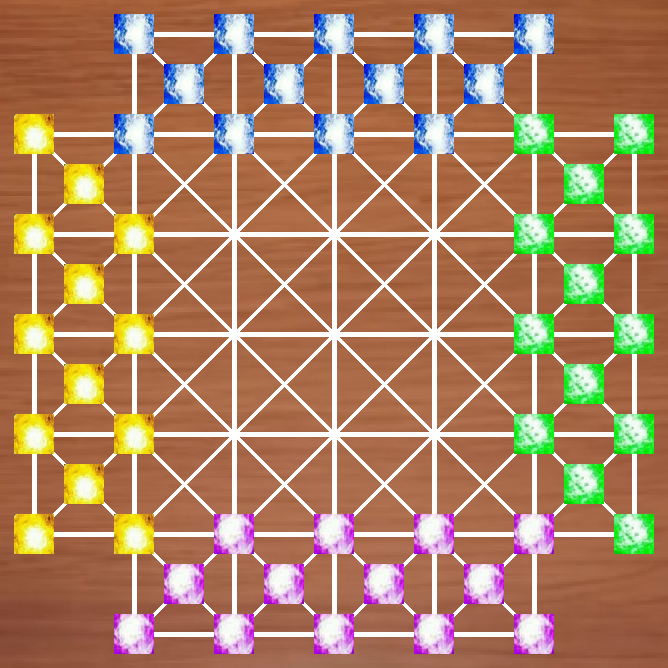
\includegraphics[width=0.52\linewidth]{figures/board_4p.png}
  \caption{Starting position of the 4-player mode (screenshot taken
  directly from the game): a 7{\texttimes}7 board with eight corner cells
  removed, forming a near-octagonal shape balanced for four directions of
  advance; four sides Blue, Green, Purple, and Yellow with 13 pieces each.
  Exact coordinates and starting positions in
  Appendix~\ref{app:multistart}.}
  \label{fig:multiboard}
\end{figure}

\subsection{2-Player Mode}
A 5{\texttimes}5 vertex board. 14 pieces per side (10 vertex + 4 centre).
Colours: Yellow and Green. This is the mode modelled in full in
Appendix~\ref{app:formal} and that uses classic Minimax Alpha-Beta
(Section~\ref{sec:ai}).

\subsection{3-Player Mode}

\begin{figure}[H]
  \centering
  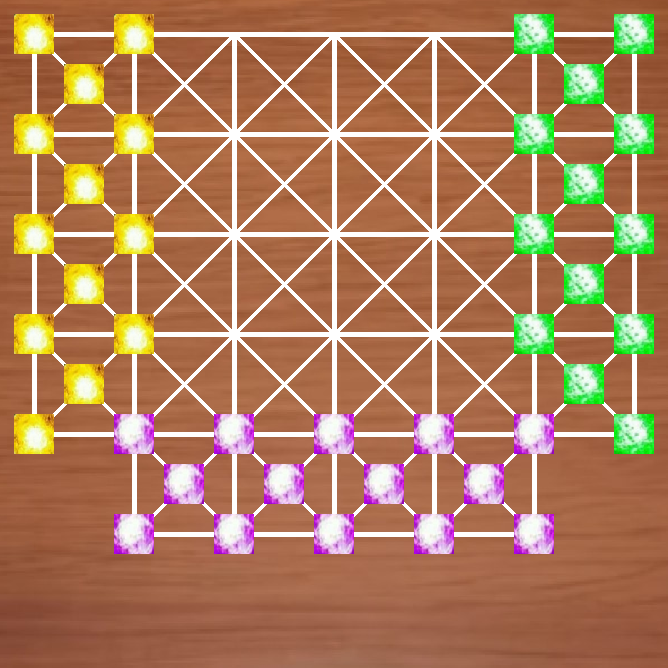
\includegraphics[width=0.52\linewidth]{figures/board_3p.png}
  \caption{Starting position of the 3-player mode (screenshot taken
  directly from the game): a 7{\texttimes}6 board with four cells removed at
  the two top corners; three sides Yellow, Green, and Purple. The
  configuration is \emph{unbalanced}---two sides have 13 pieces and the
  third has 14 (Appendix~\ref{app:multistart}).}
  \label{fig:board3p}
\end{figure}

A 7{\texttimes}6 board with the 4 top corner cells removed. Two sides have
13 pieces and the third side has 14 pieces (exact configuration and the
asymmetry note in Appendix~\ref{app:multistart}). Colours: Yellow, Green,
and Purple. This mode introduces \emph{coalition dynamics}: a player must
consider not only attacking a direct opponent but also avoiding creating an
advantage for a third opponent. Because the score is no longer fully
opposed between two sides, the AI switches to Paranoid Minimax
(Section~\ref{sec:ai})---the pessimistic assumption that the two remaining
opponents coordinate against the player.

\subsection{4-Player Mode}
A 7{\texttimes}7 board with 8 corner cells removed, 13 pieces per side.
Colours: Blue, Green, Purple, and Yellow. Four players create a complex
web of relationships; victory usually comes from holding a neutral position
and then striking decisively once the opponents have worn one another down.
